	\begin{subfigure}[b]{0.4\textwidth}
		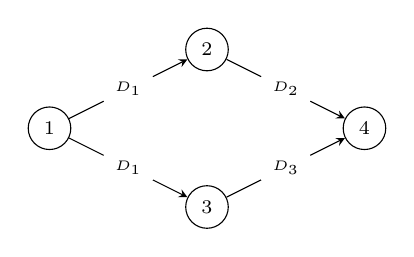
\begin{tikzpicture}
			\begin{scope}[every node/.style={circle,thin,draw}]
				\node (1a) at (+0+0,+0+0)	{\scriptsize $1$};
				\node (2a) at (+2+0,+1+0)	{\scriptsize $2$};
				\node (3a) at (+2+0,-1+0)	{\scriptsize $3$};
				\node (4a) at (+4+0,-0+0)	{\scriptsize $4$};
				
			\end{scope}

			\begin{scope}[>={stealth[black]},
				every node/.style={fill=white,circle},
				every edge/.style={draw=black,thin}]
				\path [->] (1a) edge node {\tiny $D_{1}$} (2a);
				\path [->] (1a) edge node {\tiny $D_{1}$} (3a);
				\path [->] (2a) edge node {\tiny $D_{2}$} (4a);
				\path [->] (3a) edge node {\tiny $D_{3}$} (4a);			
 			\end{scope}
		\end{tikzpicture}
		\subcaption{}
		\label{fig-STN}
	\end{subfigure}
	~
	\begin{subfigure}[b]{0.4\textwidth}
\begin{tikzpicture}
			\begin{scope}[->,>=stealth',shorten >=1pt,auto,
                semithick, scale = 1, transform shape,
                every node/.style={circle,thin,draw}]
				\node (z) at (-1.5,+1.5)	{\scriptsize $z$};
				
				\node (1a) at (+0+0,+0+0)	{\scriptsize $s_{1p}$};
				\node (2a) at (+2+0,+1+0)	{\scriptsize $s_{2p}$};
				\node (3a) at (+2+0,-1+0)	{\scriptsize $s_{3p}$};
				\node (4a) at (+4+0,-0+0)	{\scriptsize $s_{4p}$};
				
				\node (1b) at (+0+0.0,+0+3.0)	{\scriptsize $s_{1p'}$};
				\node (2b) at (+2+0.0,+1+3.0)	{\scriptsize $s_{2p'}$};
				\node (3b) at (+2+0.0,-1+3.0)	{\scriptsize $s_{3p'}$};
				\node (4b) at (+4+0.0,-0+3.0)	{\scriptsize $s_{4p'}$};				
			\end{scope}

			\begin{scope}[>={stealth[black]},
				every node/.style={fill=white,circle},
				every edge/.style={draw=black,thin}]
				
				% z1 arcs
				\path [<-] (z) edge[bend right=15] node {\tiny $0$} (1a);
				\path [->] (z) edge[bend left=15] node {\tiny $0$} (1a);
				\path [<-] (z) edge[bend right=15] node {\tiny $0$} (1b);
				\path [->] (z) edge[bend left=15] node {\tiny $0$} (1b);	
						
				% ij arcs for scenario p
				\path [<-] (1a) edge node {\tiny $-d_{1p}$} (2a);
				\path [<-] (1a) edge node {\tiny $-d_{1p}$} (3a);
				\path [<-] (2a) edge node {\tiny $-d_{2p}$} (4a);
				\path [<-] (3a) edge node {\tiny $-d_{3p}$} (4a);
				
				% ij arcs for scenario p'
				\path [<-] (1b) edge node {\tiny $-d_{1p'}$} (2b);
				\path [<-] (1b) edge node {\tiny $-d_{1p'}$} (3b);
				\path [<-] (2b) edge node {\tiny $-d_{2p'}$} (4b);
				\path [<-] (3b) edge node {\tiny $-d_{3p'}$} (4b);	

							
				% s1p - w - s1p'
				\path [->] (1a) edge[bend right=8] node[] {\tiny $w$} (1b);
				\path [<-] (1a) edge[bend left=8] node[] {\tiny $w$} (1b);
				
				% s2p - w - s2p'
				\path [dotted,<->] (2a) edge[bend left=15] node[pos=0.7] {\tiny $w$} (2b);
				
				% s3p - w - s3p'
				\path [dotted,<->] (3a) edge[bend right=15] node[pos=0.3] {\tiny $w$} (3b);
				
				% s4p - w - s4p'
				\path [->] (4a) edge[bend right=8] node[] {\tiny $w$} (4b);
				\path [<-] (4a) edge[bend left=8] node[] {\tiny $w$} (4b);
			\end{scope}
		\end{tikzpicture}
		\subcaption{}
		\label{fig-STN}
	\end{subfigure}
